\chapter{Stand der Technik}
\label{ch:StandDerTechnik}

Mit dem zunehmenden Einfluss von Computern auf die Gesellschaft wurde auch die Interaktion von Mensch und Computer ein immer wichtigerer Bestandteil unseres Alltags. Innerhalb der letzten Jahrzehnte wurde auf diesem Gebiet stetig geforscht und die verfügbaren Technologien weiterentwickelt, mit dem Ziel, die Interaktion von Mensch und Computer so natürlich wie möglich zu gestalten. Diese Entwicklung erstreckte sich von der ursprünglichen Kommunikation mittels Maus und Tastatur, über Touchscreens und Virtual Reality Systeme, bis hin zu Sprachsteuerungen von elektronischen Endgeräten. Vor diesem Hintergrund hat auch das Interesse an Gestenerkennung als zusätzliches natürliches Kommunikationsmittel zugenommen. \\
Bei Gestenerkennungssystemen kann man grundsätzliche zwischen zwei verschiedenen Arten der Gestenerkennung unterscheiden: Bei der \textit{gerätebasierten Gestenerkennung} werden die Bewegungen eines Nutzers durch Beschleunigungs- oder Positionssensoren wahrgenommen und einer Geste zugeordnet. Bei dieser Art der Gestenerkennung muss der Nutzer die Sensorik in irgendeiner Form am Körper tragen, damit die Bewegungsmuster richtig aufgezeichnet werden können. Dabei kann z.B. ein Handschuh wie der CyberGlove II des Unternehmens CyberGlove Systems (siehe \reffig{fig:CyberGlove}) oder ein einfacher Controller wie bei der Spielekonsole Wii von Nintendo (siehe \reffig{fig:WiiController}) zum Einsatz kommen. \\
\begin{figure}[H]
	\centering
	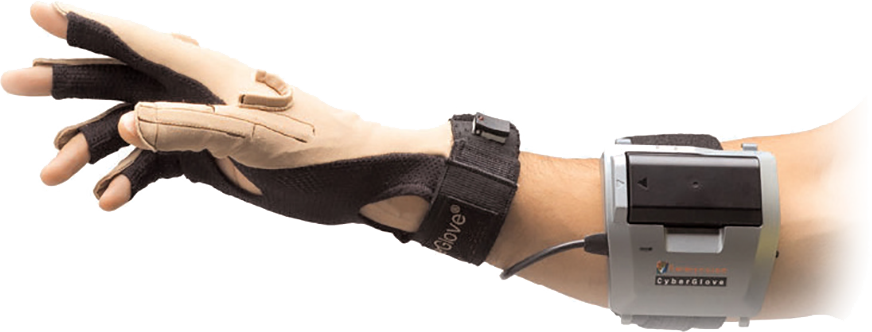
\includegraphics[scale=0.4]{../figures/CyberGlove.png}
	\caption{Der CyberGLove II von CyberGlove Systems. Er enthält verschiedene Sensoren, unter Anderem Biegesensoren für die Finger, sowie Sensoren zur Detektion der Drehung des Handgelenks. \source{\url{http://www.cyberglovesystems.com/cyberglove-ii/}}}
	\label{fig:CyberGlove}
\end{figure}
\begin{figure}[h]
	\centering
	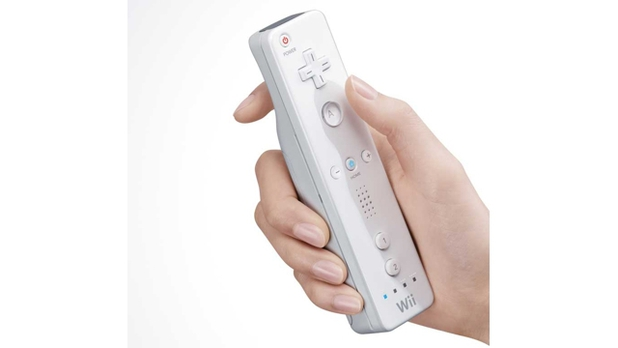
\includegraphics[scale=0.5]{../figures/WiiController.jpg}
	\caption{Ein Controller der Nintendo Spielekonsole Wii. Die Erkennung der Bewegungen des Spielers erfolgt mit Hilfe von Positions- und Beschleunigungssensoren. \source{\url{https://www.chip.de/artikel/Nintendo-Wii-Test-2_140216386.html}}}
	\label{fig:WiiController}
\end{figure}
\noindent
\textit{Kamerabasierte Gestenerkennungsverfahren} nutzen externe Systeme, die die Bewegungen des Nutzers beobachten und Aufnahmen von dessen Bewegungsabläufen erstellen. Dabei werden meistens Kamerasysteme eingesetzt. Auf die aufgenommenen Bilddaten werden dann verschiedene Bildrekonstruktionsverfahren sowie Bildanalyseverfahren angewendet, um die Gestendaten zu extrahieren. Nachdem die Gestendaten extrahiert wurden, erfolgt ein Abgleich mit einer Datenbank, in der verschiedene Aufnahmen von verschiedenen Gesten gespeichert sind. Dieser Datenbankabgleich erlaubt dann letztendlich die Zuordnung der Geste. Ein Beispiel für ein System, das auf diese Weise arbeitet, ist die Kinect Erweiterung für die XBox-Spielekonsole von Microsoft (siehe auch \reffig{fig:MSKinect}).
\begin{figure}[h]
	\centering
	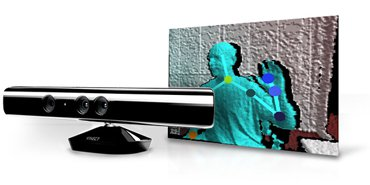
\includegraphics[scale=0.5]{../figures/MSKinect.jpg}
	\caption{Das kamerabasierte Gestenerkennungssystem Kinect von Microsoft. Es werden Aufnahmen des Nutzers gemacht, die nach einer Analyse mit einer Datenbank abgeglichen werden, um die Geste zu zuordnen. \source{\url{https://blogs.microsoft.com/ai/kinect-for-windows-game-on-for-commercial-use/}}}
	\label{fig:MSKinect}
\end{figure}
Beide Arten von Gestenerkennungssystemen werden aktuell eingesetzt. Allerdings haben beide Verfahren gewisse Nachteile: So erfordern gerätebasierte Gestenerkennungssysteme immer Sensorik am Körper des Nutzers, was sich in alltäglichen Situationen häufig als unkomfortabel erweist. Demgegenüber können kamerabasierte Gestenerkennungssysteme nur in ausreichend hellen Umgebungen arbeiten, ein Einsatz bei Dunkelheit oder in dunklen Räumen ist meist nicht möglich. Dazu können Probleme mit den Bilderkennungsverfahren auftreten, sofern die Farbe der Hand und die Hintergrundfarbe sehr ähnlich sind. Bei einer zu geringen Auflösung des Kamerasystems müssen sich die Gesten stark unterscheiden, damit sie von den Bildanalyseverfahren extrahiert werden können und selbst dann kann das System nur solche Gesten erkennen, die in der Datenbank vorhanden sind. Zudem sind Datenbankabfragen und Vergleiche mit den darin gespeicherten Daten häufig sehr rechenaufwändig, was sich als problematisch erweisen kann, falls eine Echtzeit Erkennung der Gesten gefordert ist. Eine Anbindung an die Datenbank erfordert zudem einen ständigen Internet Zugang oder alternativ große Mengen an Speicherplatz, um die für den Abgleich benötigten Gestendaten lokal zu speichern. Insbesondere für den Einsatz in eingebetteten Systemen, wie z.B. in der Automobil-Industrie sind diese beiden Gestenerkennungsverfahren nur bedingt geeignet: Gerätebasierte Gestenerkennungssysteme benötigen externe Sensorik am Körper des Nutzers, die mit dem eingebetteten System kommunizieren und Daten austauschen muss. Dabei ist in eingebetteten System häufig die Kommunikation über externe Schnittstellen sehr zeitaufwändig. Eingebettete Systeme dürfen zudem oft nur einen geringen Energieverbrauch aufweisen. Das erschwert den Einsatz von den Kamerasystemen, die von kamerabasierten Erkennungsverfahren benötigt werden. Zudem muss die für die Bilderkennung bzw. -analyse eingesetzte Software plattformunabhängig sein, damit sie auch im Rahmen des eingebetteten Systems eingesetzt werden kann. \\
Genau an dieser Schnittstelle zu eingebetteten Systemen soll der Gestikulaser eingesetzt werden können. Durch die Verwendung von robusten elektronischen Bauteilen in Kombination mit 8-bit Mikrocontrollern benötigt der Gestikulaser nur wenig Energie. Die kompakte und modulare Bauweise, auf die in \refsec{sec:Oktokommander} und \refsec{sec:Detektormodul} noch genauer eingegangen wird, erlaubt den Einsatz in unterschiedlichen Größenmaßstäben, da der Gestikulaser bei Bedarf einfach erweitert werden kann. Da die für die Gestenerkennung benötigten mathematischen Modelle (siehe dazu auch \refsec{sec:Software}) für die Anwendung individuell offline antrainiert werden, benötigt das System im Live-Betrieb vergleichsweise wenig Speicherplatz, was es ebenfalls für den Einsatz in eingebetteten Systemen qualifiziert.